Os resultados obtidos englobam a prototipação das telas da aplicação mobile que em momentos futuras será transformada em web com o objetivo de transformar em responstivo, os Diagramas de Caso de Uso e de Redes, além da Modelagem Lógica e Conceitual do Banco de Dados e do Modelo de Negócios Canvas.

\subparagraph*{\textbf{Prototipação do Figma}}

Na \cref{fig:tela-inicial}, demonstra a tela inicial, onde o usuário é direcionado para a tela de login/cadastro para poder ser utilizado.

\begin{figure}[!htb]
\centering
\SetCaptionWidth{\ifbool{@LayoutA}{0.7}{0.72}\linewidth}
\caption{Tela Inicial}%
\label{fig:tela-inicial}

\includegraphics[width = 0.4\textwidth]{Imagens/TELA INICIAL.png}
\SourceOrNote{Autoria Própria}
\end{figure}

\newpage

Na \cref{fig:tela-principal}, é demonstrada a tela principal que mostra os tanques que o usuário registra. Em cada tanque, é possível observar um botão. Esse botão é utilizado para a escolha manual ou automático da alimentação dos camarões. Nos tanques, é possível realizar a edição dos cadastros de cada tanque. 

\begin{figure}[!htb]
\centering
\SetCaptionWidth{\ifbool{@LayoutA}{0.7}{0.72}\linewidth}
\caption{Tela Principal}%
\label{fig:tela-principal}
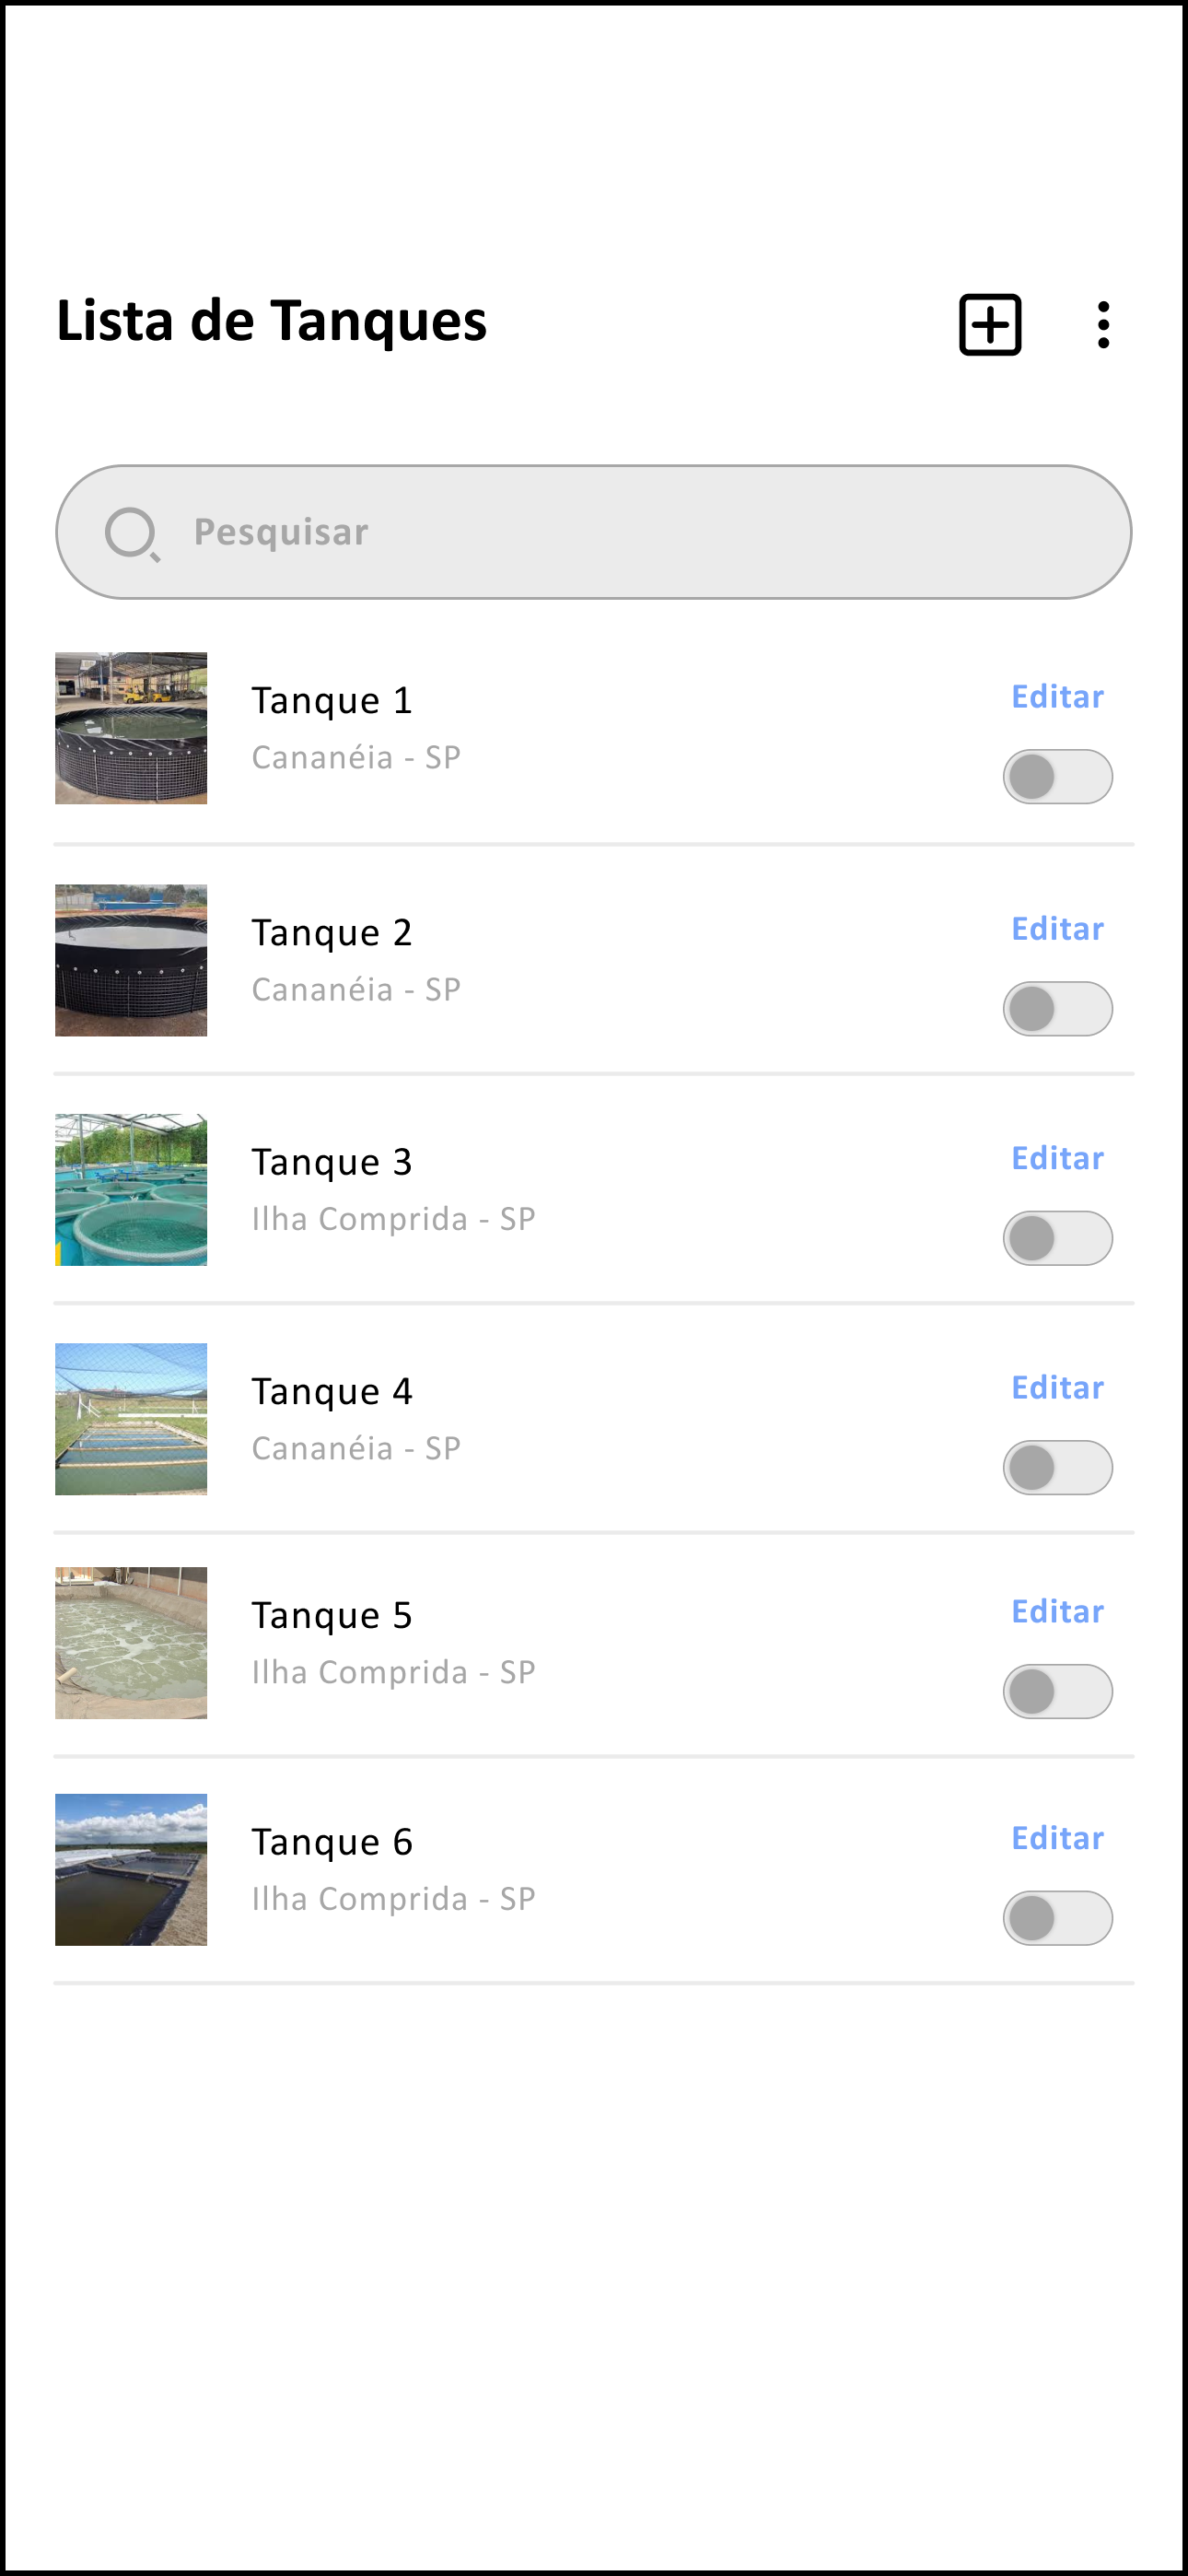
\includegraphics[width = 0.4\textwidth]{Imagens/LISTA DE TANQUES.png}
\SourceOrNote{Autoria Própria}
\end{figure}

\newpage

Na \cref{fig:tela-opções}, é demonstrada as opções que podem ser utilizadas, como Perfil em que poderá realizar a visualização de seu perfil; Notificações para visualizar todas as notificações enviadas; Meu Sítio para verificar as informações sobre o sítio do usuário e Relatório Geral em que o usuário irá selecionar determinada data para visualizar um relatório sobre os tanques e os camarões para comparações.

\begin{figure}[!htb]
\centering
\SetCaptionWidth{\ifbool{@LayoutA}{0.7}{0.72}\linewidth}
\caption{Mais Opções}%
\label{fig:tela-opções}
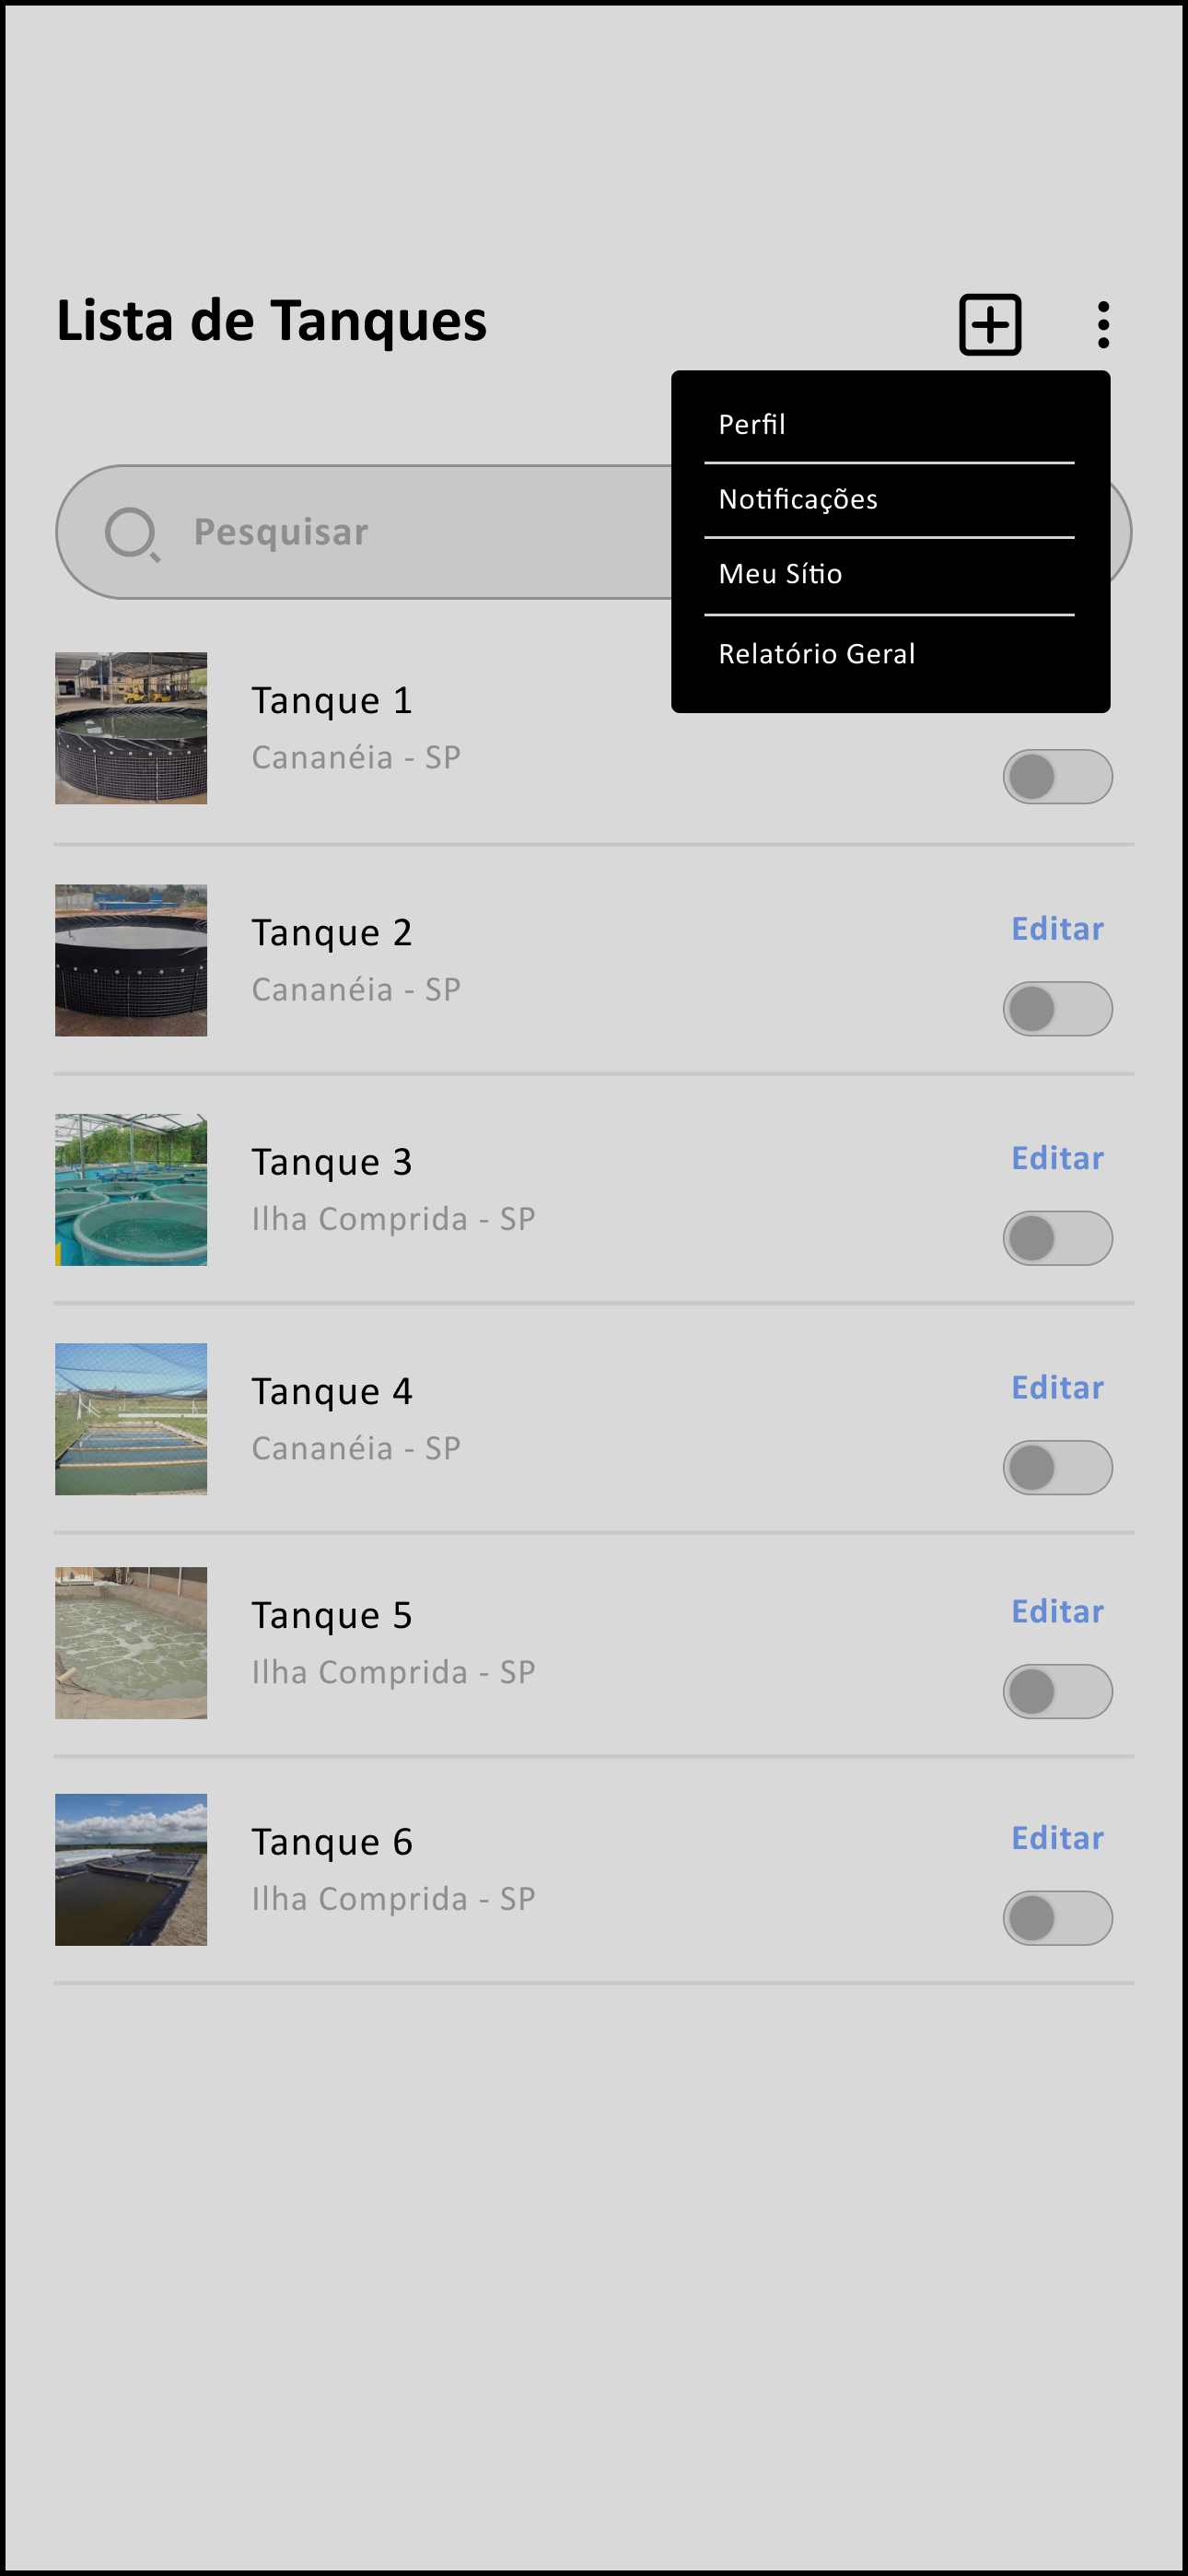
\includegraphics[width = 0.4\textwidth]{Imagens/MAIS OPÇÕES.png}
\SourceOrNote{Autoria Própria}
\end{figure}

\newpage

Na \cref{fig:tela-cativeiro}, é demonstrada a tela de cadastro de cada tanque, onde é selecionado o código de identificação do cativeiro, código de identificação do sítio e a data em que foi realizada a instalação do sistema.

\begin{figure}[!htb]
\centering
\SetCaptionWidth{\ifbool{@LayoutA}{0.7}{0.72}\linewidth}
\caption{Cadastro de Cativeiro}%
\label{fig:tela-cativeiro}
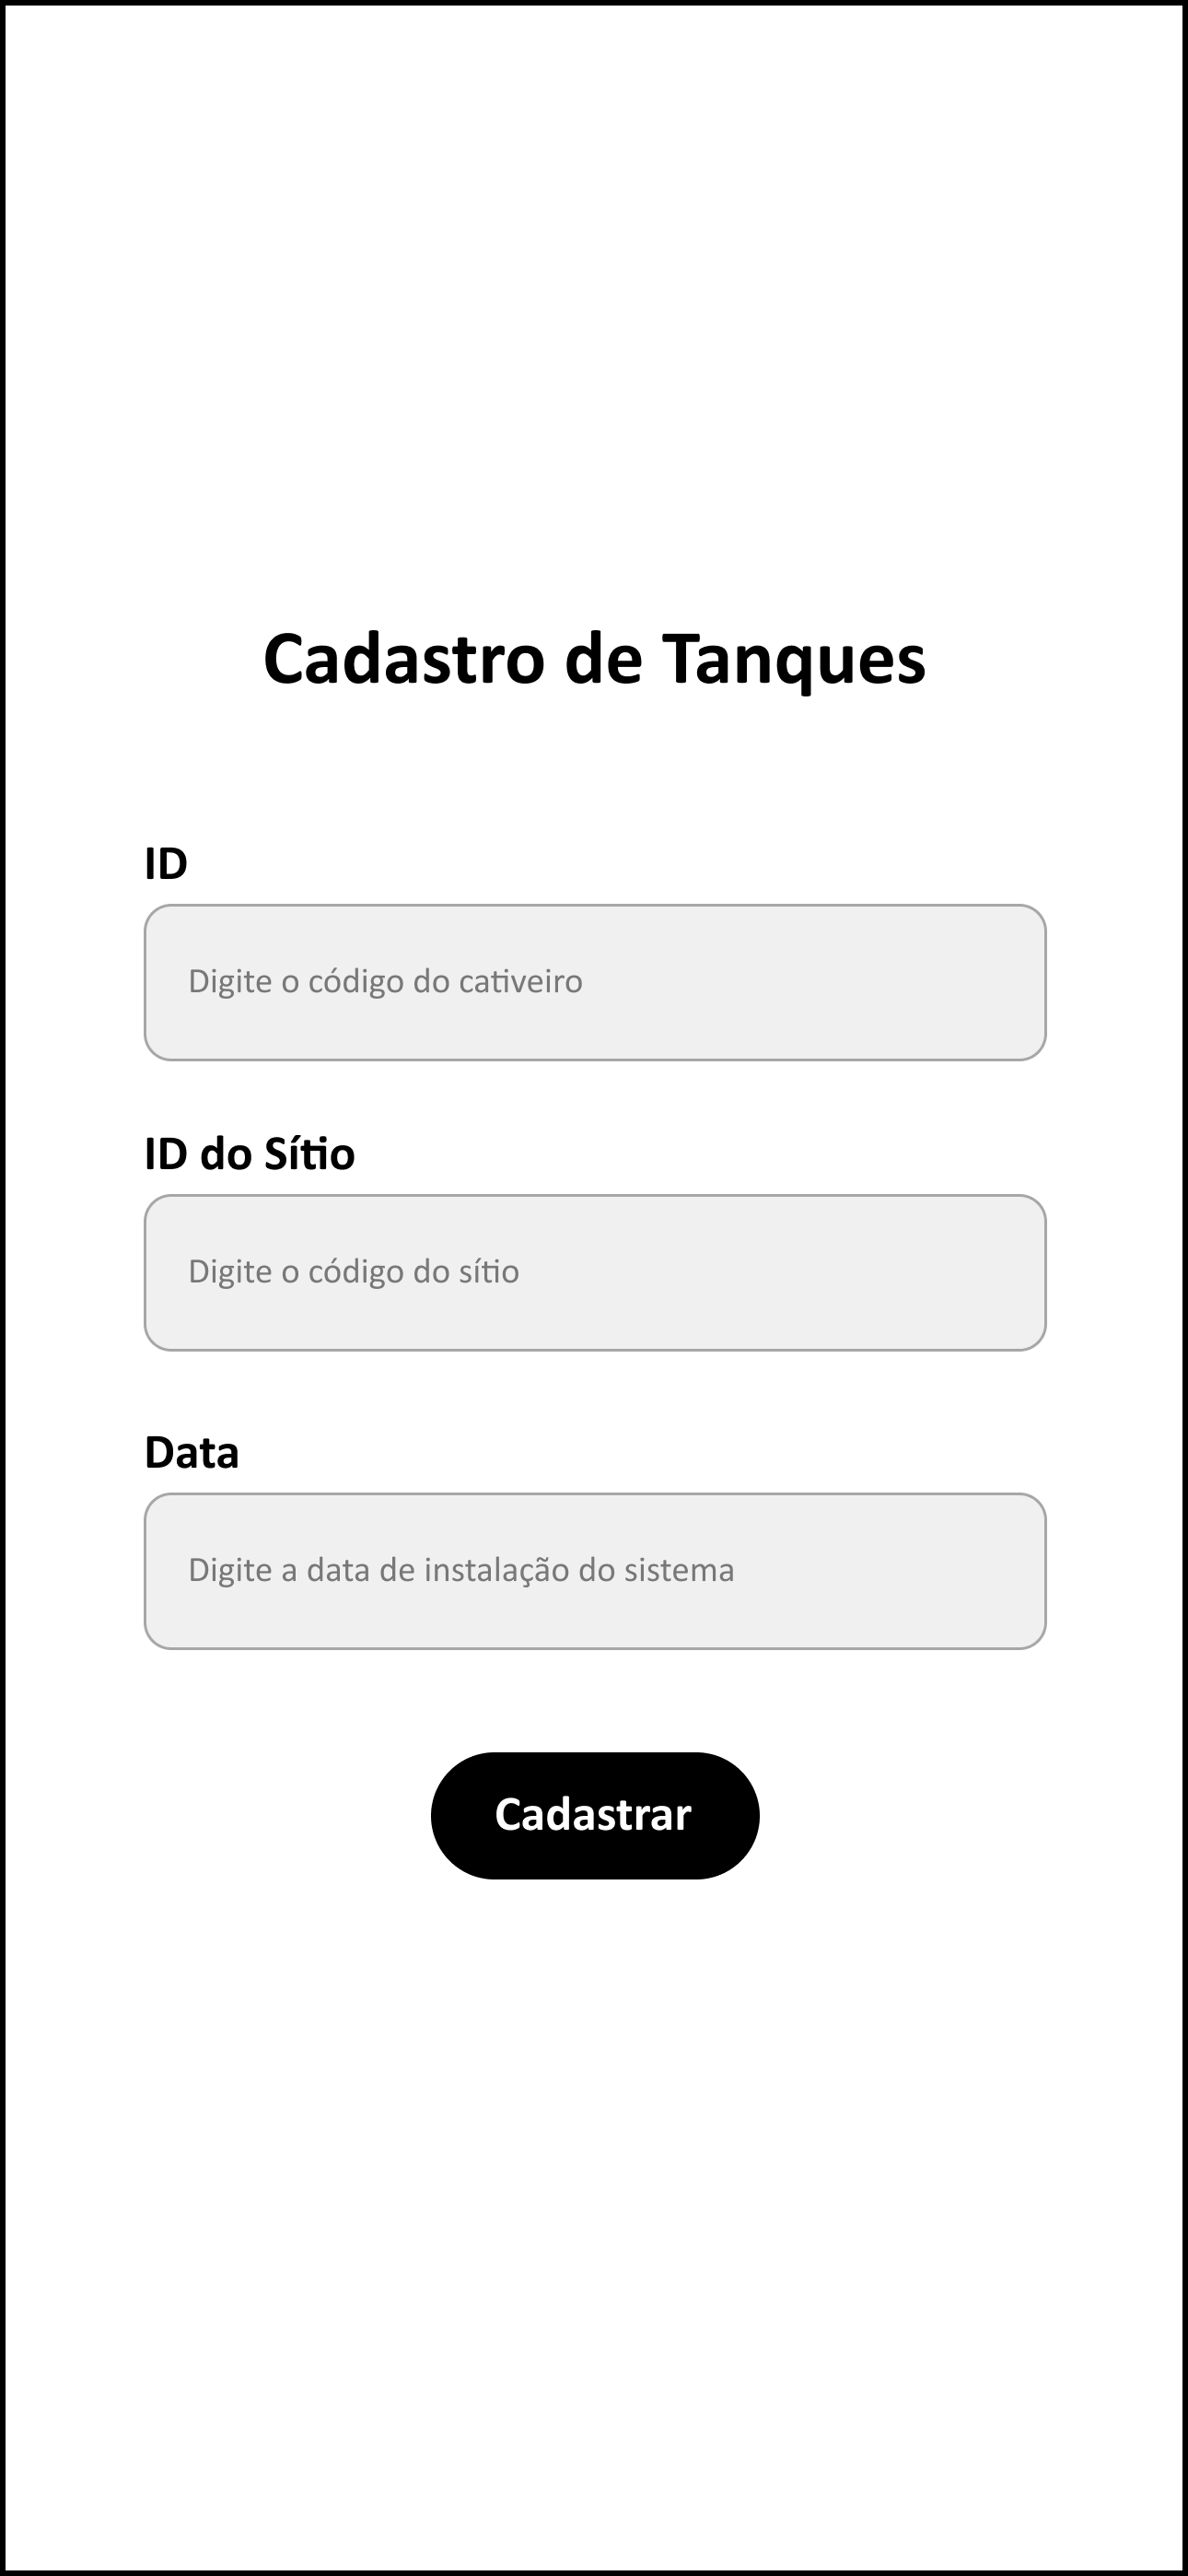
\includegraphics[width = 0.4\textwidth]{Imagens/CADASTRAR CATIVEIRO.png}
\SourceOrNote{Autoria Própria}
\end{figure}

\newpage

Na \cref{fig:tela-dashboard}, é representada a tela de dashboard, esta tela pode ser visualizada após selecionar um tanque para verificar informações. Nesta tela, é possível verificar a temperatura do cativeiro, o pH, a amônia e dentre outras informações como camarões. É possível verificar um gráfico com registro de temperatura e pH de datas recentes.

\begin{figure}[!htb]
\centering
\SetCaptionWidth{\ifbool{@LayoutA}{0.7}{0.72}\linewidth}
\caption{Dashboard}%
\label{fig:tela-dashboard}
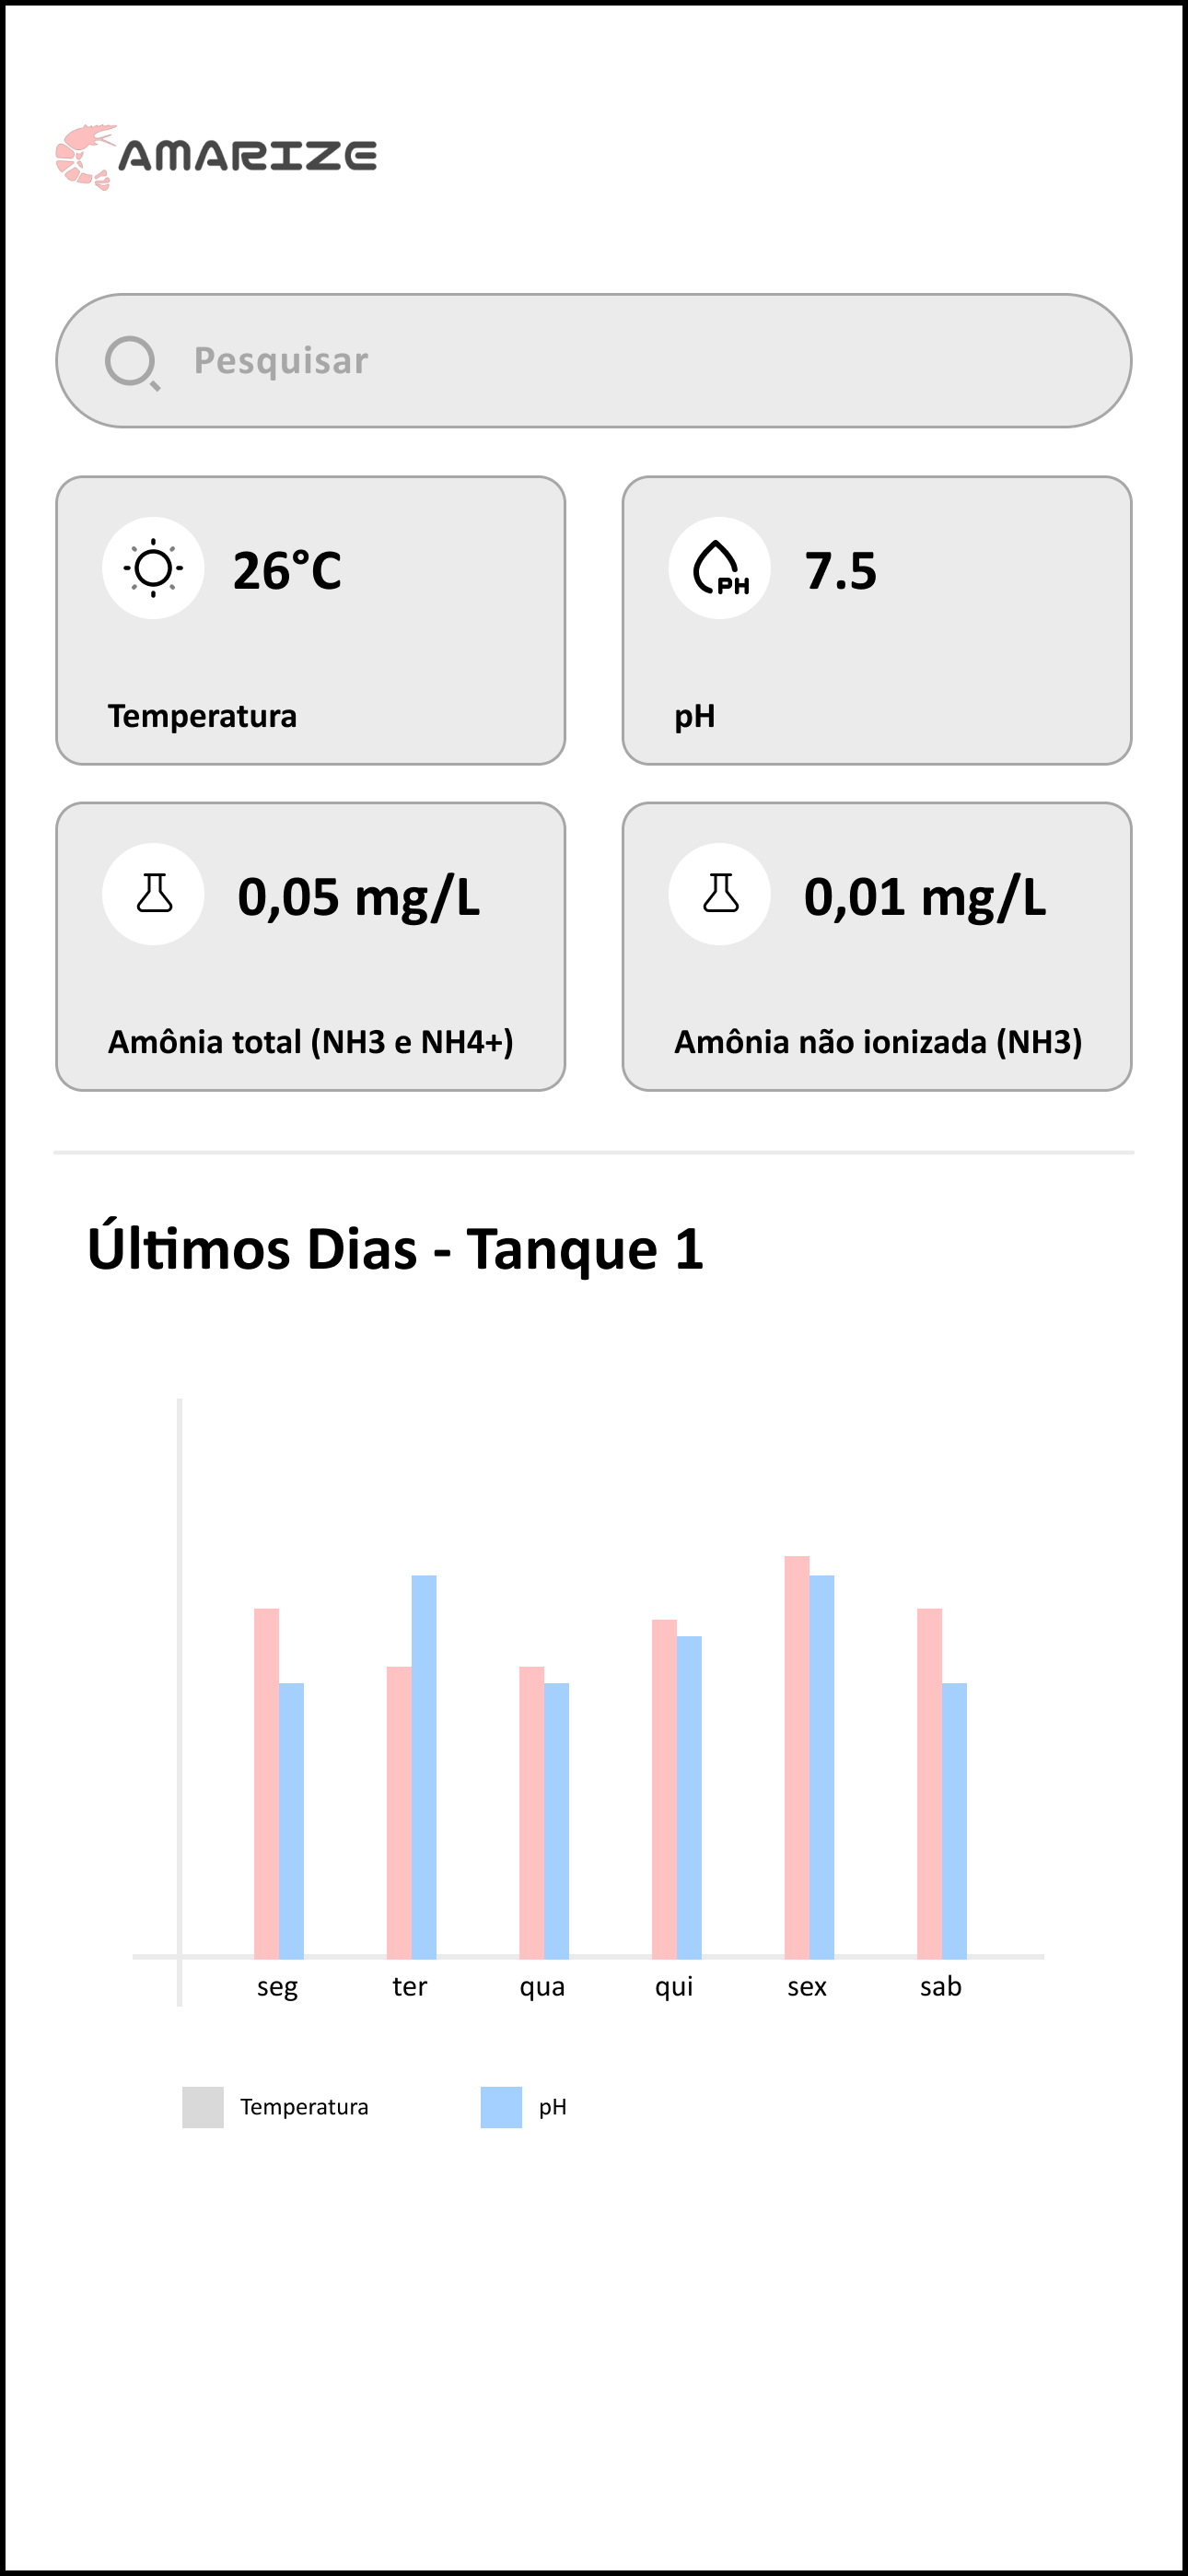
\includegraphics[width = 0.4\textwidth]{Imagens/DASHBOARD.png}
\SourceOrNote{Autoria Própria}
\end{figure}

\newpage

\subparagraph*{\textbf{Diagrama de Caso de Uso}}

Com o Diagrama de Caso de Uso (DCU), é possível verificar as interações entre o usuário, visto como o carcinicultor, e o sistema. Essas interações incluem desde a realização da conta até a analise completa de cada funcionalidade do sistema, como relatório geral, visualização dos tanques e utilização do modo automático de alimentação.

\begin{figure}[!htb]
\centering
\SetCaptionWidth{\ifbool{@LayoutA}{0.7}{0.72}\linewidth}
%
\label{fig:caso-uso}
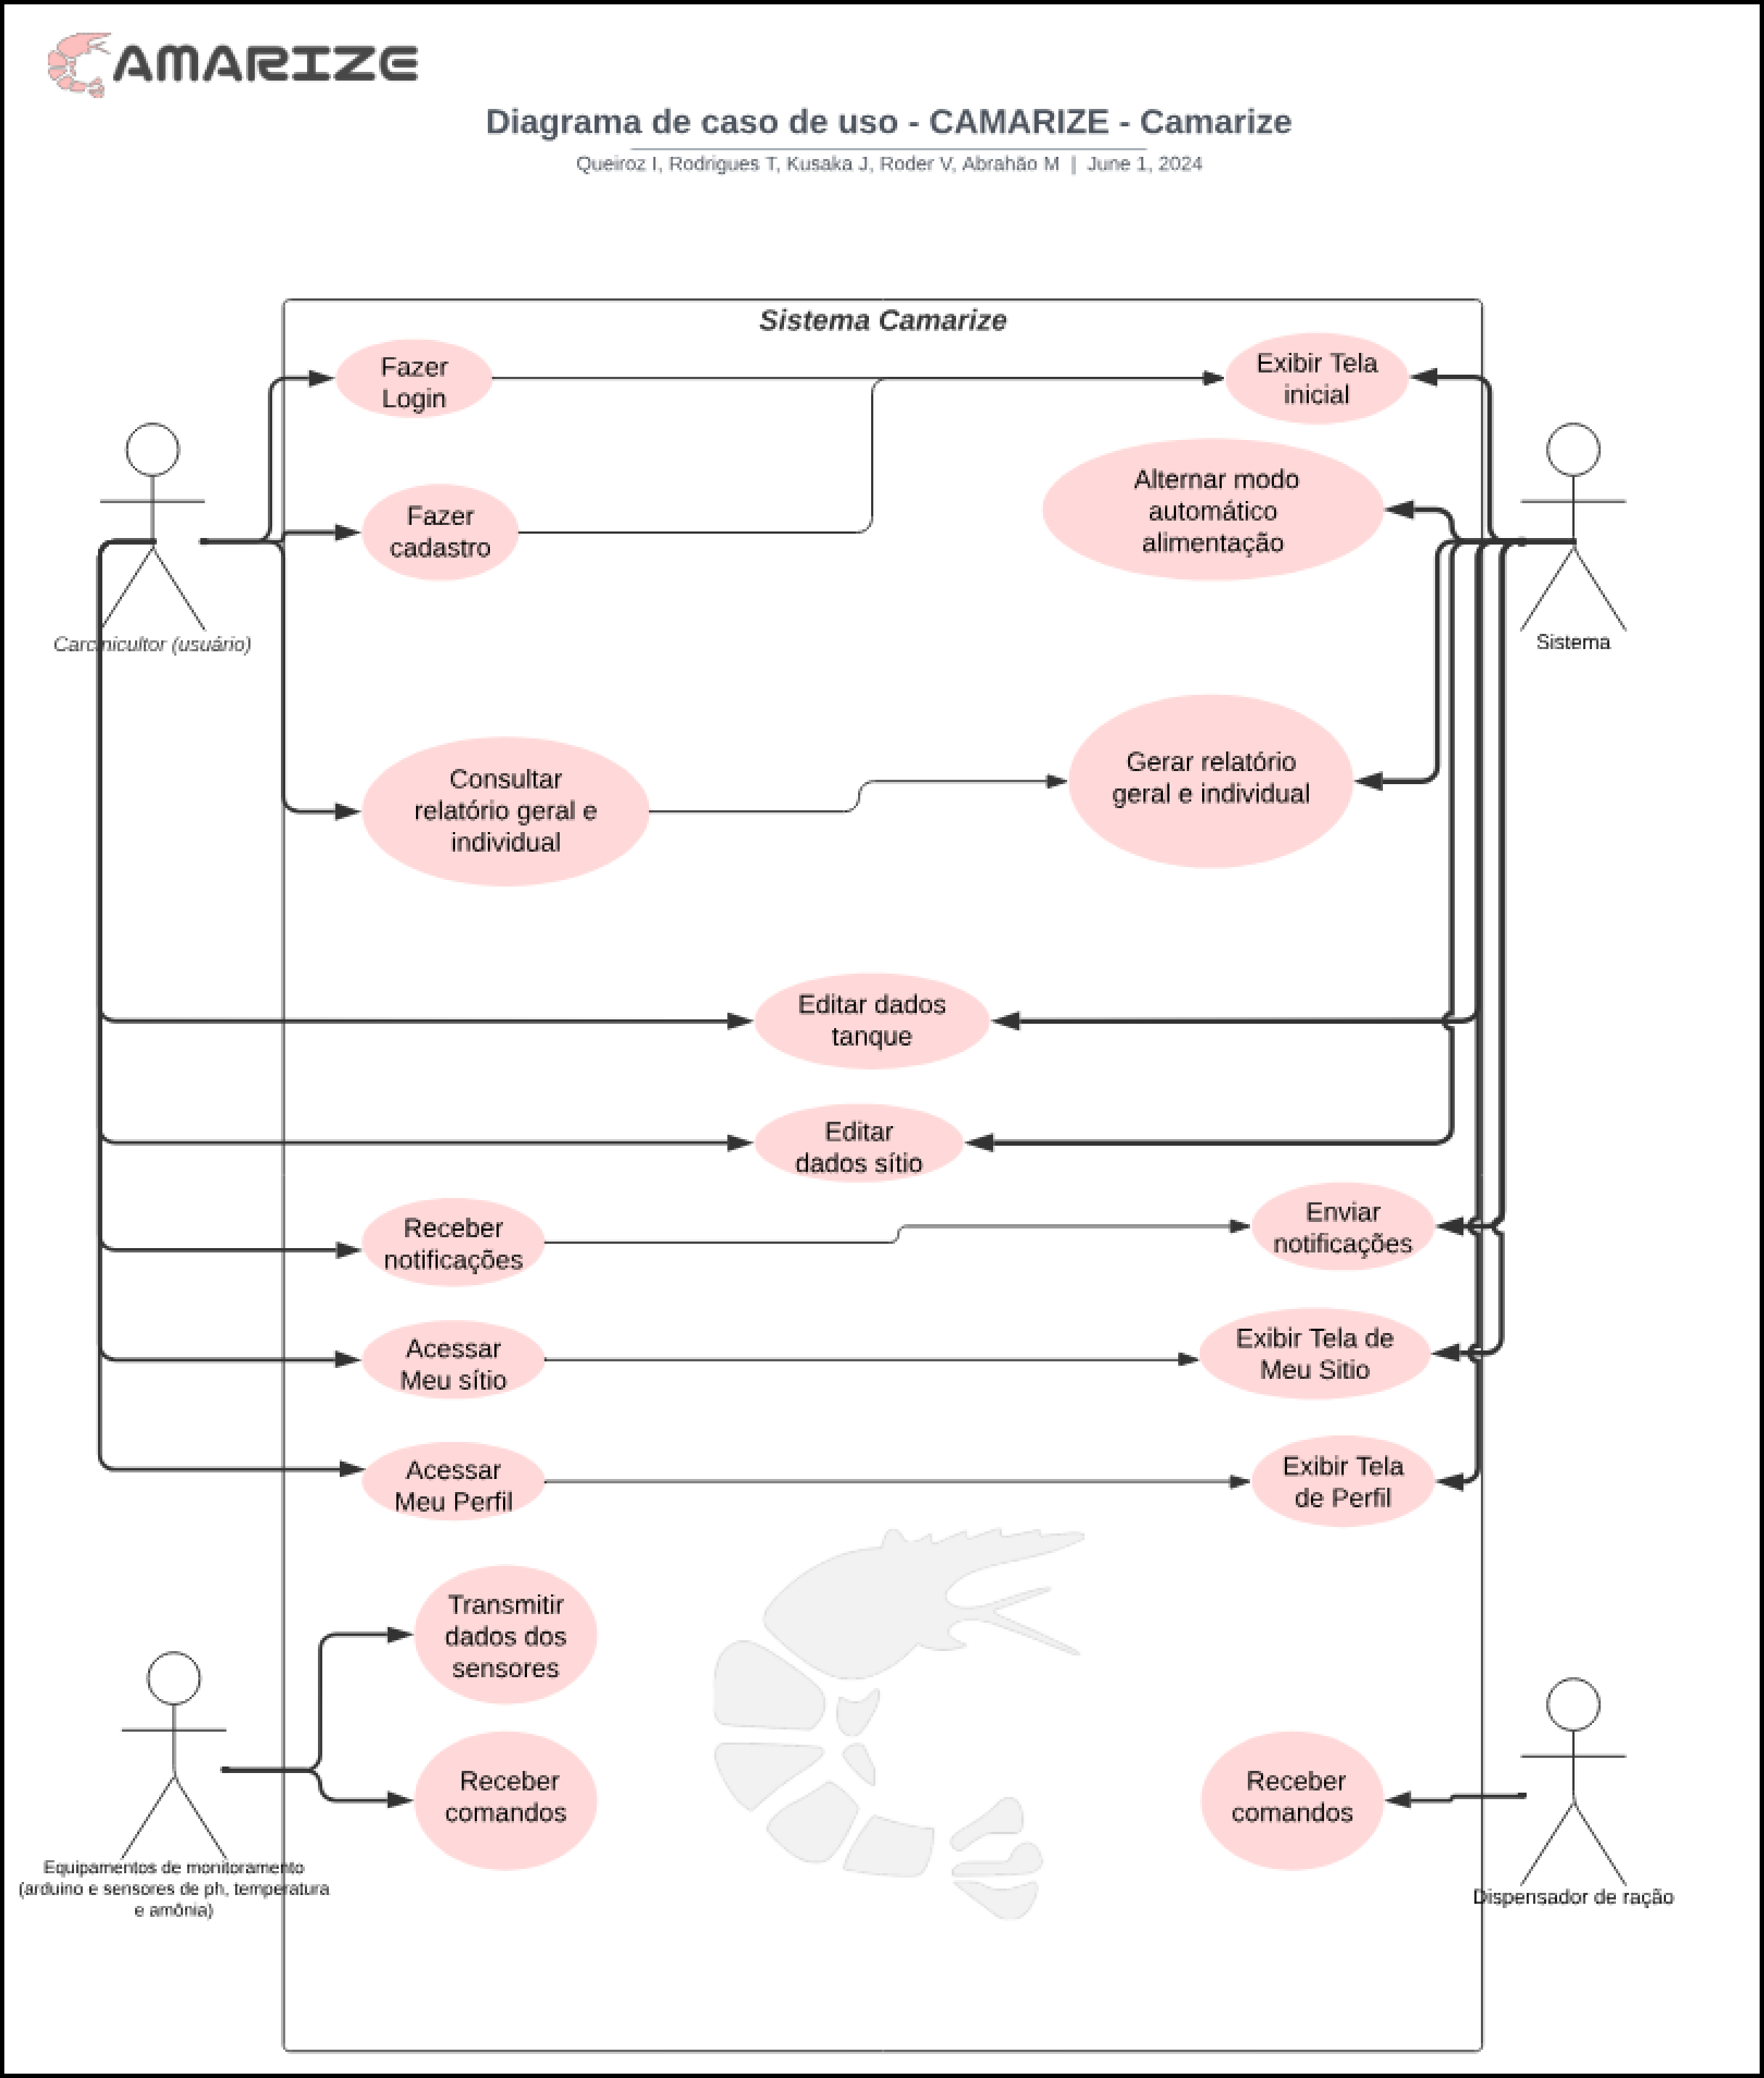
\includegraphics[width = 1.3\CaptionWidth]{Imagens/Caso de Uso.png}
\SourceOrNote{Autoria Própria}
\end{figure}

\newpage

\subparagraph*{\textbf{Diagrama de Redes}}

Por meio do Diagrama de Redes, é realizado a representação visual das redes de computadores e telecomunicações. Para o sistema, irá possuir duas etapas: Monitoramento e Alimentação. 

Na etapa de monitoramento, cada tanque estará equipado com um Arduino conectado a três sensores: medidor de temperatura, de pH e amônia. 

Na etapa de automatização da alimentação, será utilizado um dispensador de ração com uma abertura na parte inferior, equipado com um motor para controle da abertura e um sensor de nível com os parâmetros pré-definidos anteriormente para determinar a quantidade ideal de ração a ser liberada no tanque. Em ambas as etapas, irá possuir comunicação via Wi-fi com o servidor central que estará na sala de monitoramento.

\begin{figure}[!htb]
\centering
\SetCaptionWidth{\ifbool{@LayoutA}{0.7}{0.72}\linewidth}
\caption{Diagrama de Redes}%
\label{fig:redes}
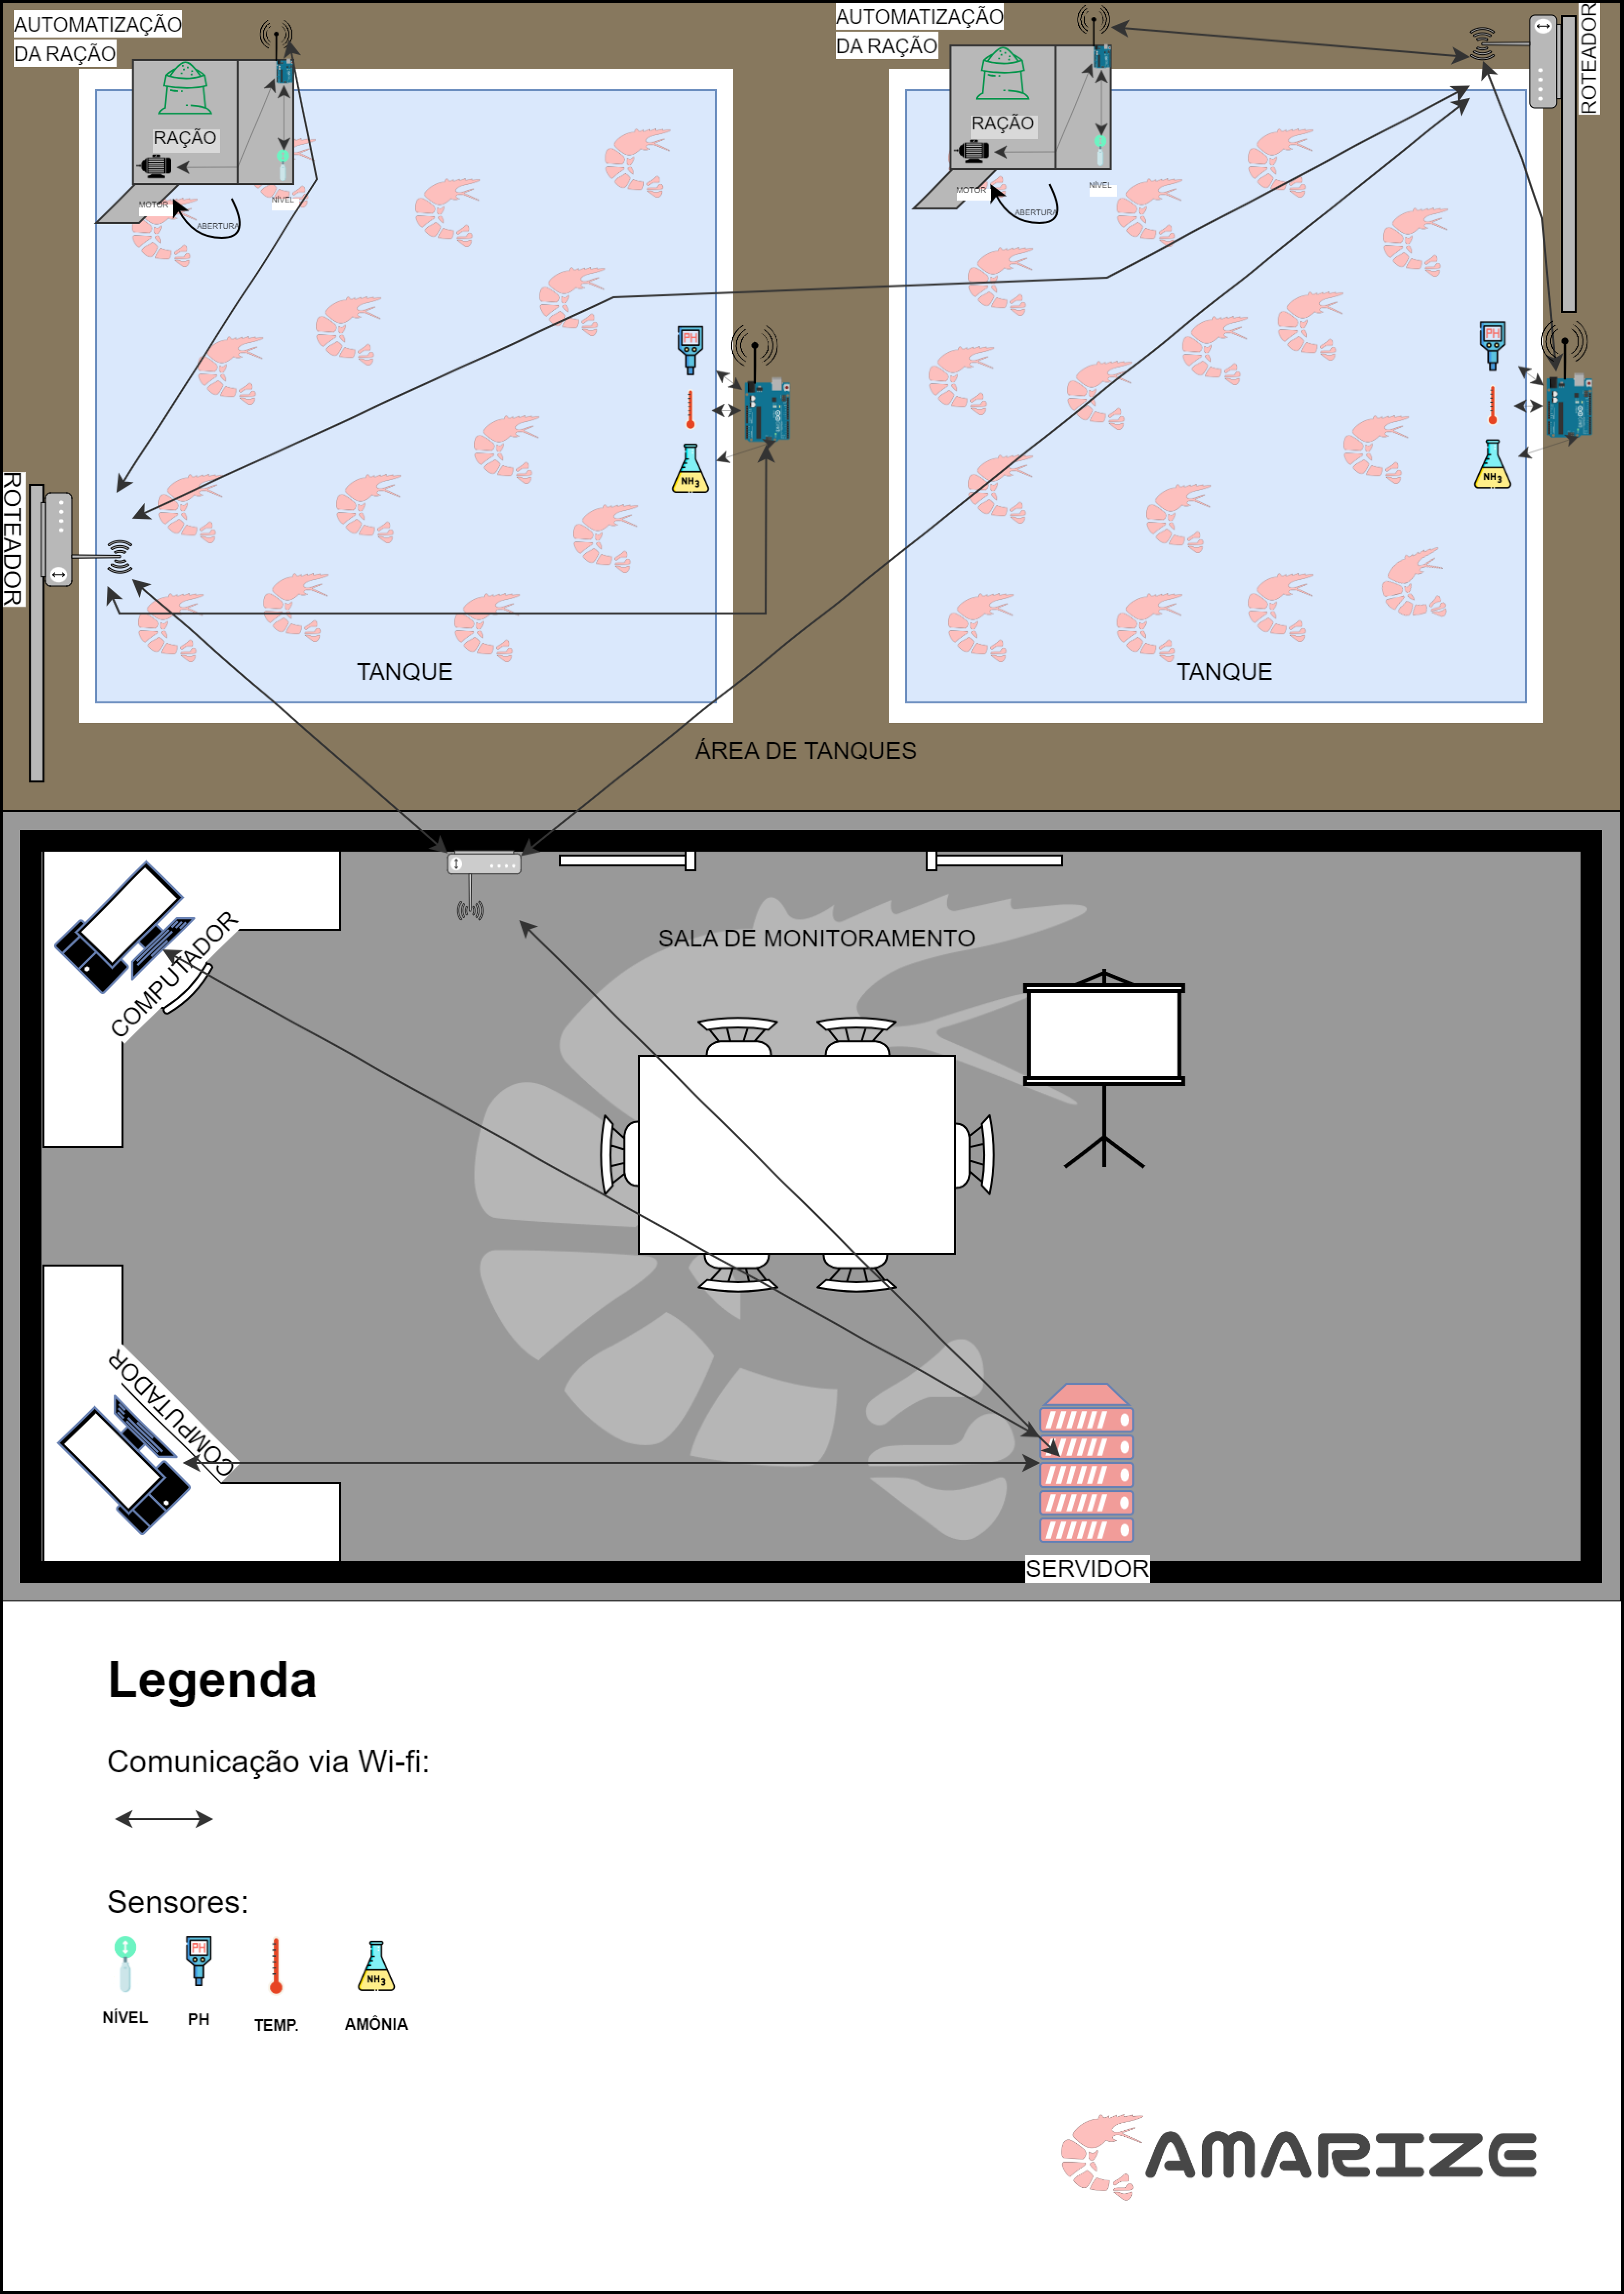
\includegraphics[width = 0.6\textwidth]{Imagens/Diagrama de Redes.png}
\SourceOrNote{Autoria Própria}
\end{figure}

\newpage

\subparagraph*{\textbf{Modelagem Lógica e Conceitual do Banco de Dados}}

O banco de dados tem um papel de extrema importância para as informações, sendo necessário para guardar, organizar e recuperar dados. O Modelo Lógico e Conceitual são maneira de demonstrar a eficiência de um banco de dados.

A modelagem conceitual e lógica, representada na \cref{fig:conceitual} e \cref{fig:logico}, demonstra a funcionalidade do programa e do que será aplicado no banco de dados. A visão gráfica do banco de dados se demonstra algo fundamental, por conta que proporciona o máximo de detalhes com extrema clareza, apresentando as relações entre as entidades.

No modelo conceitual, Camarões está ligado com Cativeiro por meio de Tipos de Camarões, apresentando característica como espécie e peso. Com os Cativeiros fazendo parte de Sítios, pode-se realizar o Monitoramento por meio de Sensores e controlar a Alimentação dos camarões. O Monitoramento possui Temperatura, pH e Amônia fazendo assim o registro de cada um. Alimentação possui o horário que foi realizado a alimentação e a quantidade de alimento fornecida para cada Cativeiro.

No modelo lógico, é apresentado uma representação mais concreta do banco de dados, demonstrando as tabelas, entidades, chaves primárias e estrangeiras e seus relacionamentos.

\begin{landscape}
\begin{figure}[!htb]
\SetCaptionWidth{\ifbool{@LayoutA}{0.7}{0.72}\linewidth}
\caption{Modelo Conceitual}%
\label{fig:conceitual}
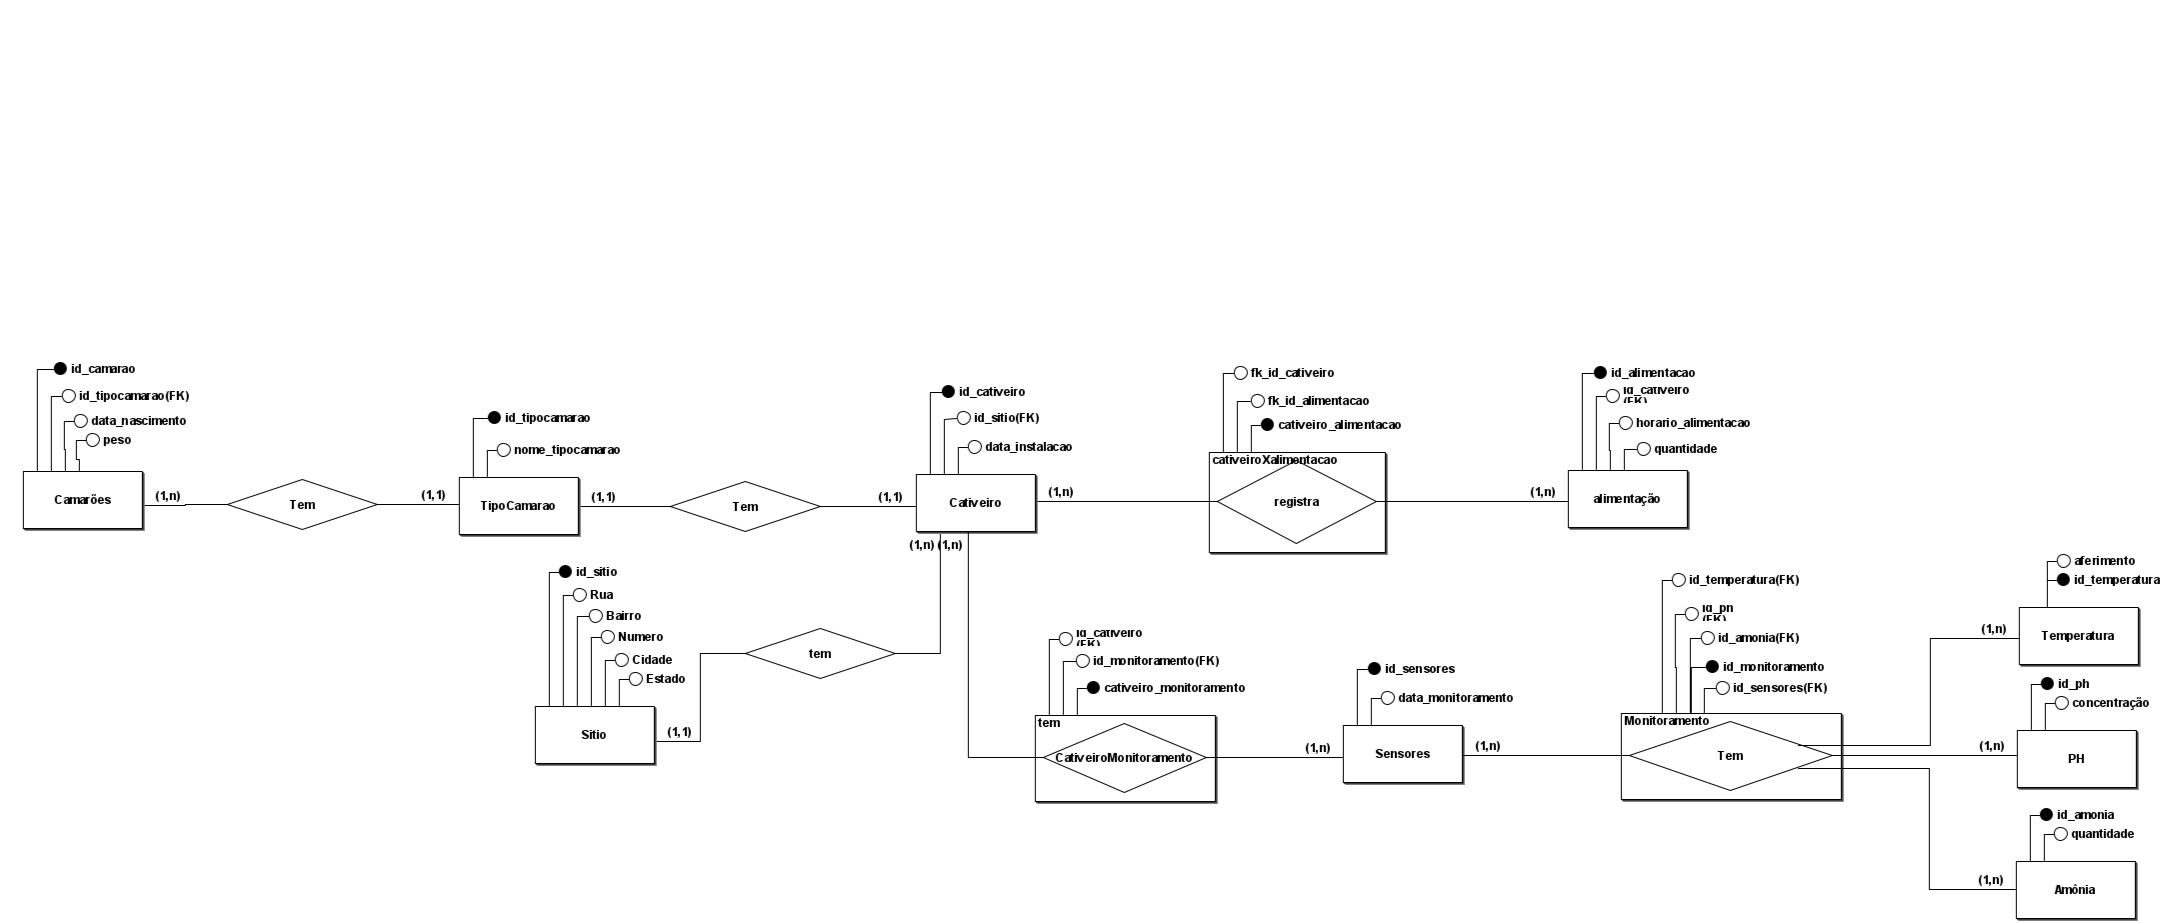
\includegraphics[width = 1.5\CaptionWidth]{Imagens/Modelo Conceitual.png}
\SourceOrNote{Autoria Própria}
\end{figure}

\begin{figure}[!htb]
\SetCaptionWidth{\ifbool{@LayoutA}{0.7}{0.72}\linewidth}
\caption{Modelo Lógico}%
\label{fig:logico}
\includegraphics[width = 1.5\CaptionWidth]{Imagens/Modelo Lógico.png}
\SourceOrNote{Autoria Própria}
\end{figure}

\end{landscape}

\subparagraph*{\textbf{Modelo de Negócio Canvas}}

O modelo de negócios Canvas foi utilizado para análise econômica do sistema. Por meio do Canvas foi possível identificar os Parceiros, Recursos e Atividades Chaves, nossas Propostas de Valor, Segmento de Mercado, nossa Fonte de Renda e Estrutura de Custos.

